% Proposta de Trabalho de Conclusão de Curso
% Curso de Ciência da Computação — Universidade de Passo Fundo
% Autor: Igor Zanette — Matrícula: 198862
% Orientador: Prof. Rafael Rieder

\documentclass[alpha-refs,brazilian,oneside]{upf-ccc}

%----------------------------------------------------------------
% Pacotes adicionais
%----------------------------------------------------------------
\usepackage{graphicx}
\usepackage{multirow}
\usepackage{nicefrac}
\usepackage{epstopdf}
\usepackage{chngcntr}
\counterwithout{figure}{chapter}
\counterwithout{table}{chapter}
\counterwithout{equation}{chapter}
\counterwithout{footnote}{chapter}
\usepackage{notoccite}
\usepackage{adjustbox}
\usepackage{enumitem}
\usepackage{threeparttable}
\usepackage{tikz}
\usetikzlibrary{shapes.geometric, arrows.meta, positioning, fit, backgrounds}

%----------------------------------------------------------------
% Ajuste de quebra de linha: evita palavras invadindo a margem
%----------------------------------------------------------------
\tolerance=1000
\emergencystretch=3em
\hyphenpenalty=200
% Hifenização correta de termos técnicos recorrentes
\hyphenation{
  apti-dão edá-fica frutí-feras macieira maracu-jazeiro
  mirti-leiro nogueira-pecã quivi-zeiro espe-cia-lista
  con-cor-dân-cia infe-rência reco-men-dação inter-pre-tação
  Embra-pa Comis-são fer-tili-dade adu-bação cala-gem
  pro-pri-edades microba-cias}

%----------------------------------------------------------------
% Dados do trabalho (OBRIGATÓRIO)
%----------------------------------------------------------------
\author{Igor Zanette}

\title{SIRAS: Sistema de Interpretação e Recomendação Agronômica de Solo}
      {SIRAS: a Soil Interpretation and Agronomic Recommendation System}

\tipotrabalho{\monografia}

\orientador{Rafael Rieder}

%----------------------------------------------------------------
% Início do documento
%----------------------------------------------------------------
\begin{document}

%----------------------------------------------------------------
% Sumário
%----------------------------------------------------------------
\tableofcontents

%----------------------------------------------------------------
% Seções da proposta
%----------------------------------------------------------------
\chapter{RESUMO}\label{chap:resumo}

Este trabalho propõe o desenvolvimento do SIRAS --- Sistema de Interpretação
e Recomendação Agronômica de Solo ---, um sistema especialista baseado em
regras para interpretação automática de análises químicas e físicas de solo,
geração de recomendações técnicas de correção e manejo, e estimativa de aptidão
agrícola para 61 culturas e grupos de culturas com relevância para o Rio Grande do Sul, abrangendo
culturas de grãos, hortaliças, tubérculos, frutíferas, erva-mate, tabaco e cana-de-açúcar.
A motivação decorre da observação, em contextos de assistência técnica rural e
crédito agrícola, de que a ausência de ferramentas computacionais acessíveis e
integradas compromete a qualidade das decisões técnicas e financeiras no setor
agropecuário. A revisão de literatura abordará os parâmetros químicos e físicos
do solo relevantes para a interpretação agronômica, os critérios de calagem e
adubação vigentes para o RS conforme o Manual de Calagem e Adubação da Sociedade
Brasileira de Ciência do Solo, os fundamentos de sistemas especialistas baseados
em regras e os sistemas computacionais correlatos existentes, como o FertFacil e
o Sistema de Avaliação de Aptidão Agrícola da Embrapa. A metodologia
caracteriza-se como pesquisa descritiva e aplicada, de abordagem quantitativa,
e prevê a estruturação da base de conhecimento a partir das normas regionais,
o projeto e a implementação dos módulos de entrada de dados, recomendação e
estimativa de aptidão, e a validação do SIRAS em três dimensões complementares:
a correção das saídas, medida pela taxa de concordância com valores de
referência calculados de forma independente, que definirá a aceitação das
hipóteses formuladas; a comparação qualitativa com ferramentas existentes; e a
avaliação de usabilidade junto ao público-alvo. Espera-se, ao final, dispor de uma ferramenta que integre recomendação
de manejo e estimativa de aptidão agrícola a partir de uma análise individual de
solo, preenchendo uma lacuna identificada nos sistemas disponíveis e contribuindo
para a tomada de decisão de técnicos, produtores e instituições financeiras que
operam com crédito rural.

\chapter{Motivação e Objetivos}\label{chap:problema}

Este capítulo apresenta a motivação que originou a proposta deste trabalho,
os objetivos geral e específicos a serem alcançados e as hipóteses de pesquisa formuladas.

\section{Motivação}

A interpretação de análises químicas e físicas de solo é uma etapa essencial
no planejamento da fertilidade e do manejo das culturas agrícolas. Trata-se de
um processo que exige elevado conhecimento técnico e atenção rigorosa, pois erros
de interpretação podem acarretar prejuízos financeiros significativos aos produtores,
seja pelo uso desnecessário de insumos, seja pela redução de produtividade decorrente
de correções insuficientes.

A complexidade desse processo advém da multiplicidade de variáveis envolvidas
--- pH, teores de macronutrientes e micronutrientes, capacidade de troca catiônica
(CTC), saturação por bases, textura do solo, entre outros \citep{Embrapa2011,
ManualCalagem2016} --- e da necessidade de correlacioná-las com as exigências
específicas de cada cultura e com as características edafoclimáticas de cada região.
Ferramentas computacionais que realizem essa correlação de forma estruturada ainda
são escassas no contexto do produtor e do técnico gaúcho, especialmente no que
diz respeito à integração entre recomendações de manejo e estimativas de aptidão
agrícola para culturas específicas \citep{Hofig2015, EmbrapaAptidao2025}.

Nesse contexto, o autor deste trabalho acumulou experiência profissional tanto
na prestação de assistência técnica a produtores rurais, com contato direto com
laudos de análise de solo e recomendações de correção e adubação, quanto no
atendimento bancário a carteiras de produtores rurais, em processos vinculados
à liberação de crédito rural. Nessa última atividade, observa-se que projetos
agrícolas submetidos às instituições financeiras podem apresentar inconsistências
nas recomendações técnicas, evidenciando a necessidade de instrumentos que apoiem
a validação dessas informações de maneira objetiva e rastreável.

Diante desse cenário, identificou-se a oportunidade de desenvolver o
\textbf{SIRAS} --- \textbf{S}istema de \textbf{I}nterpretação e \textbf{R}ecomendação
\textbf{A}gronômica de \textbf{S}olo ---, uma ferramenta computacional capaz de:
(i)~interpretar automaticamente dados de análises de solo; (ii)~gerar recomendações
técnicas de correção e manejo; e (iii)~estimar a aptidão agrícola de culturas
específicas em uma determinada área. O SIRAS poderia auxiliar técnicos e produtores
no processo de tomada de decisão, reduzir erros de interpretação e servir de apoio
na análise e validação de projetos agrícolas.

Iniciativas como o FertFacil, sistema desenvolvido e disponibilizado para
técnicos e produtores do RS, SC, MS e Paraguai, demonstram que a automação do
processo de recomendação de adubação e calagem é tecnicamente viável e tem gerado
resultados concretos no campo \citep{Tiecher2016}. No entanto, ferramentas dessa
natureza concentram-se na geração de recomendações de correção e adubação, não
contemplando a estimativa da aptidão agrícola da cultura escolhida frente às
condições edáficas da área. Em escala mais ampla, a Embrapa desenvolveu o Sistema
de Avaliação de Aptidão Agrícola das Terras \citep{EmbrapaAptidao2025}, voltado
a levantamentos exploratórios regionais, o que o torna inadequado para a avaliação
individualizada de uma área específica a partir dos dados de uma análise de solo.
Conforme apontado por \cite{Hofig2015}, esse sistema é mais adequado para
análises em âmbito regional e não indica práticas de manejo para os diferentes
tipos de utilização, sendo necessárias adaptações para estudos mais detalhados.
Constata-se, portanto, uma lacuna entre as ferramentas disponíveis: existem
sistemas que recomendam correção do solo, e existem métodos que avaliam aptidão
em escala regional, mas não há, no contexto das ferramentas acessíveis ao produtor
e ao técnico do RS, uma solução que integre ambas as perspectivas a partir de uma
análise individual de solo. Esse é o diferencial do SIRAS.

%-------------------------------------------------------------------
\section{Objetivo Geral}\label{sec:obj_geral}

Desenvolver e avaliar o SIRAS --- Sistema de Interpretação e Recomendação
Agronômica de Solo ---, um sistema especialista baseado em regras projetado
para interpretar dados de análises químicas e físicas de solo, gerar
recomendações técnicas de correção e manejo, e estimar a aptidão agrícola
para um conjunto abrangente de culturas de interesse regional, considerando
os critérios técnicos vigentes para o estado do Rio Grande do Sul.

%-------------------------------------------------------------------
\section{Objetivos Específicos}\label{sec:obj_espec}

\begin{itemize}[leftmargin=5em]

  \item \textbf{Revisar a literatura} sobre os principais parâmetros utilizados
    na interpretação de análises de solo, abrangendo aspectos químicos e físicos,
    suas correlações com o desempenho das culturas agrícolas contempladas pelo
    SIRAS, e os critérios de calagem e adubação vigentes para o Rio Grande do Sul;

  \item \textbf{Definir critérios técnicos} para as recomendações de correção
    e manejo do solo e para a estimativa de aptidão agrícola das culturas
    contempladas, com base nos manuais e normas regionais vigentes;

  \item \textbf{Projetar e implementar} o SIRAS, incluindo os módulos de
    entrada de dados de análise de solo, processamento das recomendações
    de correção, e estimativa de aptidão agrícola por cultura;

  \item \textbf{Validar o SIRAS} quanto à correção de suas saídas, medindo
    a taxa de concordância das recomendações geradas com valores de
    referência calculados de forma independente a partir dos critérios
    técnicos vigentes;

  \item \textbf{Avaliar a contribuição e a usabilidade do SIRAS}, comparando-o
    qualitativamente às ferramentas existentes para evidenciar seu diferencial
    e aferindo a experiência de uso junto ao público-alvo.

\end{itemize}

%-------------------------------------------------------------------
\section{Hipóteses}\label{sec:hipoteses}

Com base no problema identificado e nos objetivos propostos,
formulam-se as seguintes hipóteses de pesquisa:

\begin{itemize}

  \item \textbf{H\textsubscript{0.1}:} O SIRAS \textbf{não} é capaz de gerar
    recomendações de calagem e adubação com taxa de concordância igual ou
    superior a 80\% em relação aos valores de referência derivados dos
    critérios estabelecidos no Manual de Calagem e Adubação para os estados
    do RS e SC.

  \item \textbf{H\textsubscript{1.1}:} O SIRAS \textbf{é} capaz de gerar
    recomendações de calagem e adubação com taxa de concordância igual ou
    superior a 80\% em relação aos valores de referência derivados dos
    critérios estabelecidos no Manual de Calagem e Adubação para os estados
    do RS e SC.

  \item \textbf{H\textsubscript{0.2}:} O SIRAS \textbf{não} é capaz de estimar
    a aptidão edáfica das culturas contempladas com taxa de concordância igual
    ou superior a 80\% em relação à classificação de referência construída a
    partir das exigências agronômicas descritas na literatura técnica.

  \item \textbf{H\textsubscript{1.2}:} O SIRAS \textbf{é} capaz de estimar
    a aptidão edáfica das culturas contempladas com taxa de concordância igual
    ou superior a 80\% em relação à classificação de referência construída a
    partir das exigências agronômicas descritas na literatura técnica,
    diferenciando-se dos sistemas de avaliação regional existentes por operar
    a partir de uma análise individual de solo.

\end{itemize}

A confirmação de H\textsubscript{1.1} indicará que é viável automatizar,
ao menos parcialmente, o processo de interpretação de análises de solo e
geração de recomendações para o contexto do RS. A confirmação de
H\textsubscript{1.2} demonstrará que a integração entre recomendação de
manejo e estimativa de aptidão agrícola, a partir de dados individuais
de solo, representa uma contribuição concreta do SIRAS em relação às
ferramentas atualmente disponíveis. As definições operacionais de
concordância, o conjunto de casos de teste e o procedimento de decisão
sobre as hipóteses são detalhados no \cref{chap:metodologia}.

\chapter{Revisão de Literatura}\label{chap:revisao}

Este capítulo apresenta os fundamentos teóricos e os trabalhos relacionados
que embasam o desenvolvimento de um sistema computacional para interpretação
de análises de solo e recomendação agronômica. A revisão foi conduzida
de forma narrativa, com buscas realizadas nas bases Google Scholar, SciELO,
IEEE Xplore e no repositório da Embrapa, utilizando os termos
\textit{análise de solo}, \textit{calagem e adubação}, \textit{aptidão agrícola},
\textit{expert system agriculture} e \textit{sistema especialista agronomia},
com filtros para publicações em língua portuguesa e inglesa. Foram priorizadas
publicações com abrangência para o estado do Rio Grande do Sul e trabalhos
que descrevem sistemas computacionais aplicados ao manejo da fertilidade do solo.

\section{Fundamentação Teórica}

Esta seção apresenta os conceitos teóricos que sustentam o desenvolvimento
do trabalho. São abordados os principais parâmetros das análises químicas e
físicas de solo, os critérios de calagem e adubação vigentes para o Rio Grande
do Sul, os fundamentos da avaliação de aptidão agrícola das terras e os
princípios dos sistemas especialistas baseados em regras.

\subsection{Análise Química e Física do Solo}

A análise de solo é o principal instrumento para o diagnóstico da fertilidade
e para o planejamento das práticas de manejo nutricional das culturas. Por meio
dela, determinam-se os teores de nutrientes disponíveis, a reação do solo e
atributos físicos que condicionam a produtividade das lavouras
\citep{Embrapa2011}.

Os principais parâmetros avaliados em uma análise química de solo incluem o
pH em água, que indica a acidez ou alcalinidade do meio e condiciona a
disponibilidade da maioria dos nutrientes; o teor de fósforo disponível (P);
os teores de potássio (K), cálcio (Ca) e magnésio (Mg) trocáveis; o alumínio
trocável (Al\textsuperscript{3+}), associado à toxidez em solos ácidos;
a capacidade de troca de cátions (CTC), que expressa a capacidade do solo
em reter e fornecer nutrientes; e a saturação por bases (V\%), que indica
a proporção da CTC ocupada por bases trocáveis \citep{Embrapa2011, ManualCalagem2016}.

A textura do solo, determinada pela proporção de areia, silte e argila,
constitui o principal atributo físico considerado na interpretação das análises,
pois influencia diretamente a CTC, a capacidade de retenção de água e a
resposta do solo à calagem \citep{ManualCalagem2016}. O teor de matéria orgânica
(MO) também é avaliado, dada sua contribuição para a CTC efetiva e para a
disponibilidade de nitrogênio \citep{Santos2003}. Além dos macronutrientes,
os micronutrientes --- como boro, manganês, cobre e zinco --- vêm recebendo
atenção crescente nas pesquisas regionais, com a publicação recente de
conjuntos de dados experimentais sobre sua aplicação em culturas de grãos
no Sul do Brasil \citep{FontouraEtAl2026}.

Conforme \cite{EmbrapaDoc206}, a interpretação dos resultados analíticos exige
que os valores obtidos sejam comparados a faixas de referência estabelecidas
para cada parâmetro, considerando-se o tipo de solo e a cultura de interesse.

\subsection{Calagem e Adubação para o Rio Grande do Sul}

O Manual de Calagem e Adubação para os estados do Rio Grande do Sul e de
Santa Catarina, elaborado pela Comissão de Química e Fertilidade do Solo
(CQFS/NRS-SBCS), constitui a principal referência técnica para as
recomendações de correção e fertilização no sul do Brasil
\citep{ManualCalagem2016}. O manual estabelece critérios específicos para
interpretação dos atributos do solo, métodos de cálculo da necessidade de
calagem e doses de fertilizantes para as principais culturas da região.

A calagem é a prática que visa elevar o pH do solo a níveis adequados para
o desenvolvimento das culturas, neutralizando o alumínio tóxico e elevando
a disponibilidade de cálcio e magnésio. Para a maioria das culturas de interesse
regional, o manual define um pH de referência específico, a partir do qual
o cálculo da necessidade de calagem é realizado com base na saturação por bases
atual do solo, na saturação alvo correspondente ao pH de referência da cultura,
na CTC e no poder de neutralização do corretivo \citep{ManualCalagem2016}.

A adubação fosfatada e potássica é dimensionada com base nos teores
disponíveis no solo, interpretados em classes de disponibilidade (muito baixo,
baixo, médio, alto e muito alto), e na expectativa de rendimento da cultura.
O manual fornece tabelas de recomendação individuais para cada cultura ou grupo
de culturas \citep{ManualCalagem2016}.

\subsection{Aptidão Agrícola das Terras}

A avaliação da aptidão agrícola das terras tem por objetivo classificar
as áreas de acordo com seu potencial para os diferentes tipos de uso
agropecuário, considerando as limitações impostas pelos atributos do solo
e do relevo sob diferentes níveis tecnológicos. O principal sistema utilizado
no Brasil é o Sistema de Avaliação da Aptidão Agrícola das Terras, desenvolvido
pela Embrapa, que classifica as terras em seis grupos de aptidão com base em
cinco fatores de limitação: deficiência de fertilidade, deficiência hídrica,
excesso de água, suscetibilidade à erosão e impedimentos à mecanização
\citep{EmbrapaAptidao2025}.

Conforme apontado por \cite{Hofig2015}, em estudo conduzido no município de
Cerro Grande do Sul/RS, o Sistema de Avaliação da Aptidão Agrícola das Terras
é mais adequado para análises em âmbito regional, não indicando práticas de
manejo para os diferentes tipos de utilização nem sendo projetado para a
avaliação individualizada de propriedades a partir de dados de análise de solo.
Os autores ressaltam que adaptações são necessárias para seu uso no planejamento
conservacionista de propriedades rurais, evidenciando uma lacuna metodológica
relevante para propriedades rurais de escala individual.

Uma abordagem alternativa consiste na estimativa de aptidão a partir dos
próprios parâmetros da análise de solo, cruzados com as exigências agronômicas
de cada cultura, sem considerar fatores de relevo e clima. Trata-se de uma
estimativa de aptidão edáfica, delimitada às condições de fertilidade e físicas
do solo para uma cultura específica, mais adequada à avaliação individualizada
de áreas a partir de laudos de análise.

\section{Sistemas Especialistas Baseados em Regras}

Sistemas especialistas (SE) são programas computacionais que utilizam
técnicas de inteligência artificial para reproduzir o raciocínio de um
especialista humano em um domínio específico do conhecimento, apoiando
processos de tomada de decisão, diagnóstico e recomendação
\citep{SantosEtAl1994}. Conforme \cite{SantosEtAl1994}, um sistema
especialista é constituído por três componentes fundamentais: a
\textbf{base de conhecimento}, que armazena os fatos, regras e heurísticas
do domínio; o \textbf{motor de inferência}, responsável por aplicar as
regras à base de conhecimento para derivar conclusões a partir dos dados
de entrada; e a \textbf{interface com o usuário}, que permite a comunicação
bidirecional entre o sistema e o usuário final.

Os sistemas baseados em regras do tipo SE-ENTÃO (\textit{if-then})
constituem a abordagem mais difundida para a representação do conhecimento
agronômico em sistemas computacionais. Nesse modelo, cada regra representa
um fragmento do conhecimento especialista na forma
\textit{SE} <condição> \textit{ENTÃO} <conclusão>, e o motor de inferência
percorre a base de regras para identificar quais condições são satisfeitas
pelos dados de entrada, derivando as recomendações correspondentes
\citep{Lanzer2010}.

A aplicação de sistemas especialistas na agricultura tem sido estudada em
diferentes contextos. \cite{Lanzer2010} desenvolveu um sistema especialista
baseado em regras para a classificação do uso e manejo das terras, aplicando
representação hierárquica do conhecimento~--- indicada para sistemas que lidam
com classificação~--- em um sistema de determinação de uso das terras compatível
com o sistema brasileiro. O autor destaca que a introspecção facilita o
desenvolvimento nos estágios iniciais de um sistema especialista quando as
informações para definição dos estados estão presentes nos próprios sistemas
de classificação, como é o caso do Manual de Calagem e Adubação
\citep{ManualCalagem2016}.

Em escala mais ampla, \cite{Shahzadi2016} propõem um sistema especialista
para agricultura inteligente baseado em Internet das Coisas (IoT), no qual
regras de conhecimento são alimentadas com dados coletados em tempo real por
sensores, gerando diagnósticos e recomendações preventivas para o manejo de
doenças e pragas. Embora voltado a um domínio diferente, o estudo evidencia
a viabilidade e a aplicabilidade prática de sistemas especialistas baseados
em regras para o suporte à decisão agronômica.

\section{Trabalhos Relacionados}

Esta seção apresenta os principais sistemas e ferramentas computacionais
identificados na literatura que se relacionam ao escopo do presente trabalho,
discutindo suas características, abrangência e limitações.

\textbf{FertFacil} é um sistema online e gratuito desenvolvido para estimar
a necessidade de adubação e calagem para os principais cultivos do RS, SC,
MS e Paraguai \citep{Tiecher2016}. O sistema foi desenvolvido com base nos
critérios do Manual de Calagem e Adubação e permite ao técnico ou produtor
obter recomendações de forma rápida, a partir da entrada dos resultados da
análise de solo e da cultura desejada. Atualmente o FertFacil cobre mais de
100 cultivos e é a ferramenta de escolha da Emater/RS, sendo utilizado em
mais de 480 municípios do estado. Sua principal limitação identificada é a
ausência de um módulo de estimativa de aptidão agrícola integrado ao processo
de recomendação.

\textbf{AdubaTec} é um sistema web gratuito desenvolvido pela Embrapa
Mandioca e Fruticultura em parceria com a Universidade Federal do
Recôncavo da Bahia (UFRB), voltado à recomendação de calagem e adubação
para mandioca e diversas fruteiras tropicais, com arquitetura parametrizável
que permite a incorporação de novas culturas sem modificação do código-fonte
\citep{AdubaTec2021}. O AdubaTec é baseado em manuais de recomendação
voltados ao Nordeste do Brasil, não cobrindo os critérios do Manual de
Calagem e Adubação do RS/SC, e não contempla a estimativa de aptidão
agrícola a partir da análise individual de solo.

\textbf{Sistema de Avaliação de Aptidão Agrícola das Terras da Embrapa}
\citep{EmbrapaAptidao2025} é o principal sistema de referência para
classificação do potencial produtivo das terras brasileiras. Trata-se de
um sistema voltado a levantamentos regionais em escala exploratória, baseado
em mapeamento pedológico e em fatores de limitação que incluem relevo,
clima e solo. Sua escala de análise o torna inadequado para a avaliação
individualizada de uma propriedade a partir de dados de análise de solo,
conforme discutido por \cite{Hofig2015}.

A partir do levantamento realizado, constata-se que os sistemas disponíveis
abordam, de forma separada, a recomendação de manejo do solo ou a avaliação
de aptidão agrícola em escala regional. Nenhum deles integra ambas as
perspectivas a partir de uma análise individual de solo com cobertura para
o Manual RS/SC, evidenciando uma lacuna que justifica o desenvolvimento de
uma solução específica para esse contexto.

\chapter{Metodologia}\label{chap:metodologia}

Este capítulo descreve o método que será empregado para alcançar os
objetivos propostos no \cref{chap:problema}. Inicialmente, a pesquisa é
caracterizada quanto ao seu propósito, abordagem e estilo. Em seguida,
são apresentados os materiais --- o escopo de culturas contemplado e as
tecnologias de implementação ---, a sequência de passos do método, a
estratégia de validação das hipóteses, o cronograma de execução, os
resultados esperados e as limitações do estudo.

%-------------------------------------------------------------------
\section{Caracterização da Pesquisa}\label{sec:caracterizacao}

Quanto ao propósito, esta pesquisa caracteriza-se como
\textbf{descritiva e aplicada}: descreve e estrutura um conjunto de
critérios técnicos já consolidados na literatura agronômica e aplica
esse conhecimento na construção e na avaliação de um artefato
computacional \citep{Wazlawick2014}. Quanto à abordagem, a pesquisa é
\textbf{quantitativa}, uma vez que a validação se dará pela medição
objetiva da concordância entre as saídas geradas pelo sistema e valores
de referência calculados de forma independente, evitando-se métricas
subjetivas.

Quanto ao estilo de pesquisa corrente em Computação, o trabalho
enquadra-se na \textbf{apresentação de um produto} (artefato de
software). O artefato a ser construído é um \textbf{sistema especialista
baseado em regras}, isto é, um sistema que reproduz o raciocínio de um
especialista humano em um domínio restrito por meio de uma base de
conhecimento explícita e de um motor de inferência que aplica regras do
tipo SE-ENTÃO \citep{Lanzer2010, SantosEtAl1994}. Conforme
\cite{Wazlawick2014}, o estilo de apresentação de produto exige cautela,
pois a simples demonstração de funcionamento possui baixa aceitação
científica: é necessário comparar o que foi construído com alguma
referência. Por essa razão, a validação do SIRAS não se limitará à
demonstração da aplicação: as saídas serão confrontadas com um oráculo
técnico --- os valores obtidos pela aplicação manual e independente dos
critérios do Manual de Calagem e Adubação \citep{ManualCalagem2016} ---
e o sistema será posicionado frente às ferramentas existentes
discutidas no \cref{chap:revisao}, das quais se diferencia por integrar
recomendação de manejo e estimativa de aptidão edáfica a partir de uma
análise individual de solo.

%-------------------------------------------------------------------
\section{Materiais}\label{sec:materiais}

Esta seção apresenta os materiais que delimitam e viabilizam o
desenvolvimento do SIRAS. Primeiro, define-se o \textbf{escopo de
culturas} contempladas, derivado diretamente do Manual de Calagem e
Adubação para os estados do RS e SC, que constitui a principal fonte de
conhecimento do sistema. Em seguida, descreve-se a \textbf{tecnologia de
implementação} adotada --- linguagem, framework, formato da base de
conhecimento e forma de distribuição --- e as \textbf{alternativas
tecnológicas} consideradas. Esses elementos correspondem, na metodologia
de pesquisa em Computação, aos materiais e recursos necessários à
execução do trabalho \citep{Wazlawick2014}.

\subsection{Escopo de Culturas}\label{sec:escopo}

O sistema abrangerá as culturas para as quais o Manual de Calagem e
Adubação \citep{ManualCalagem2016} disponibiliza, em seu capítulo de
recomendações, tabelas completas de adubação, totalizando
\textbf{61 culturas e grupos de culturas} organizados em seis grupos,
conforme detalhado a seguir. A contagem segue a própria organização do
Manual: cada item corresponde a uma seção de recomendação, de modo que
culturas que compartilham a mesma tabela --- como melancia e melão ---
são contabilizadas como uma única entrada. Com exceção da erva-mate,
discutida adiante, todas as culturas contempladas possuem pH de
referência definido na Tabela~5.1 do Manual, requisito do módulo de
calagem do sistema. Ficam fora do escopo: (i)~as culturas sem pH de
referência cuja lógica de calagem é incompatível com o modelo
padronizado adotado, como o arroz irrigado (cujo pH se eleva
naturalmente pela inundação), a mandioca e as espécies florestais
tolerantes à acidez; e (ii)~por delimitação de escopo, os grupos do
Manual voltados a forrageiras, palmeiras (juçara, real e pupunheira),
plantas medicinais, aromáticas e condimentares, plantas ornamentais e
sistemas especiais de produção, por estarem fora do foco de lavouras
comerciais do público-alvo do sistema.

\textbf{Culturas de grãos (21):} arroz de sequeiro, amendoim, aveia branca,
aveia preta, canola, centeio, cevada, ervilha seca e ervilha forrageira,
ervilhaca, feijão, girassol, linho, milho, milho pipoca, nabo forrageiro,
painço, soja, sorgo, tremoço, trigo e triticale. Esse grupo segue lógica
uniforme de recomendação, com tabelas de N, P e K baseadas na expectativa
de rendimento e na classe de disponibilidade dos nutrientes no solo; nas
leguminosas como soja, ervilhaca e tremoço, a adubação nitrogenada não é
recomendada em razão da fixação biológica de nitrogênio
\citep{ManualCalagem2016}.

\textbf{Hortaliças (18):} abóbora, abobrinha e moranga, alcachofra, alface,
almeirão, chicória, rúcula e salsa, alho, aspargo, berinjela, beterraba e cenoura,
brócolis e couve-flor, cebola, chuchu, ervilha, mandioquinha-salsa,
melancia e melão, nabo e rabanete, pepino, pimentão, repolho e tomate.

\textbf{Tubérculos (2):} batata e batata-doce, com tabelas completas de
N, P e K.

\textbf{Frutíferas (17):} abacateiro, ameixeira, amoreira-preta, bananeira,
caquizeiro, citros, figueira, macieira, maracujazeiro, mirtileiro, morangueiro,
nogueira-pecã, oliveira, pessegueiro e nectarineira, pereira, quivizeiro e videira.
Esse grupo apresenta complexidade adicional em relação aos demais: a adubação
é estruturada em até três fases (pré-plantio, crescimento e manutenção/produção),
e o sistema deverá adaptar as recomendações de acordo com a fase informada pelo
usuário. O fósforo e o potássio de pré-plantio seguem uma tabela compartilhada
entre todas as frutíferas (Tabela 6.5.1 do Manual), enquanto as doses de
nitrogênio e as recomendações de manutenção são específicas por espécie.

\textbf{Erva-mate (1):} cultura de expressiva relevância socioeconômica no
norte do Rio Grande do Sul. Constitui a única exceção ao critério de pH de
referência: o Manual a classifica entre as espécies tolerantes à acidez,
sem pH de referência definido, indicando a calagem apenas para o adequado
suprimento de cálcio e magnésio \citep{ManualCalagem2016}; o sistema
adotará esse tratamento diferenciado, sem cálculo de necessidade de
calagem por pH alvo. Apresenta a maior complexidade de implementação
entre as culturas contempladas: a adubação pode ocorrer em programa desde
o plantio (três fases: plantio/crescimento, formação de copa e produção) ou
em programa de recuperação de ervais já estabelecidos. A adubação de produção
é calculada com base na massa verde colhida (t/ha) e no tipo de manejo
(galho grosso retido ou retirado da área), variáveis que deverão ser informadas
pelo usuário ao selecionar essa cultura \citep{ManualCalagem2016}.

\textbf{Outras culturas comerciais (2):} cana-de-açúcar e tabaco, conforme
o agrupamento do próprio Manual. O \textbf{tabaco} é cultura de grande
importância econômica no RS e SC; as recomendações diferenciam-se entre os
tipos Virgínia e Burley, especialmente nas doses de nitrogênio e potássio,
e o sistema solicitará ao usuário o tipo cultivado ao selecionar essa
cultura. A \textbf{cana-de-açúcar} possui recomendações distintas para
cana-planta e cana-soca, com adubação nitrogenada definida pelo teor de
matéria orgânica do solo. Para ambas as culturas, o Manual estabelece pH
de referência de 6,0, com a particularidade de que a calagem é indicada
apenas quando o pH do solo for inferior a 5,5, regra que será incorporada
às regras de decisão do sistema \citep{ManualCalagem2016}.

\subsection{Tecnologia de Implementação}\label{sec:tecnologia}

O sistema será desenvolvido como uma aplicação web leve, executável
localmente em navegador, utilizando \textbf{Python}\footnote{Disponível
em: \url{https://www.python.org}.} como linguagem principal
com o microframework \textbf{Flask}\footnote{Disponível em:
\url{https://flask.palletsprojects.com}.} para a camada web, complementado por
\textbf{HTML} e \textbf{CSS} para a interface com o usuário. Essa escolha
fundamenta-se em três critérios principais: (i)~legibilidade e manutenibilidade
do código, uma vez que a lógica de regras agronômicas SE-ENTÃO em Python
resulta em código mais claro e auditável do que em linguagens de tipagem fraca;
(ii)~flexibilidade de estilização, pois o uso de HTML e CSS na interface permite
customização visual completa do formulário de entrada e do laudo de saída,
sem as limitações impostas por bibliotecas de interface nativas; e
(iii)~viabilidade para execução local, já que o Flask permite servir a aplicação
no próprio computador do usuário sem necessidade de servidor remoto ou conexão
com a internet, bastando executar o comando \texttt{python app.py} e acessar
o endereço \texttt{localhost} no navegador.

Está previsto o uso do Python na versão 3.12 (ou superior) e do Flask na
série 3.x, ambos software livre distribuído sob licenças permissivas
(PSF e BSD, respectivamente), compatíveis com o uso acadêmico e executáveis
em sistemas operacionais Windows ou GNU/Linux. Não há dependência de
serviços pagos, de banco de dados dedicado ou de conexão com a internet,
o que assegura que todos os recursos planejados estão disponíveis para a
execução do trabalho.

A lógica central do sistema --- o motor de inferência baseado em regras
SE-ENTÃO --- será implementada diretamente em Python, sem o uso de bibliotecas
externas de inferência (como Experta ou PyKE), de modo a manter o código
auditável e o comportamento das regras totalmente rastreável. As tabelas técnicas
do Manual de Calagem e Adubação \citep{ManualCalagem2016} serão armazenadas em
arquivos no formato JSON, carregados localmente pela aplicação. Essa separação
entre base de conhecimento e mecanismo de inferência é coerente com o paradigma
de sistemas especialistas descrito por \cite{Lanzer2010} e \cite{SantosEtAl1994},
e permite que as tabelas de recomendação sejam atualizadas de forma independente
da lógica de processamento. Para a geração do laudo de saída, será utilizada
a capacidade de renderização do navegador, com possibilidade de impressão
direta ou exportação em PDF pelo recurso nativo dos navegadores modernos.

Quanto à forma de distribuição, o SIRAS será disponibilizado como
\textbf{software de código aberto}, com o repositório publicado em
plataforma pública de versionamento. A forma de acesso prevista nesta
proposta é a \textbf{execução local}: o usuário obtém o código-fonte,
instala as dependências (Python e Flask) e executa a aplicação em sua
própria máquina, acessando a interface pelo navegador no endereço
\texttt{localhost}. Essa opção foi escolhida por dispensar custos de
hospedagem e por manter o controle dos dados na máquina do usuário, o
que é adequado ao escopo de uma proposta de TCC. A arquitetura web
adotada, contudo, não impede uma futura implantação em servidor remoto
--- bastaria hospedar a mesma aplicação Flask para que fosse acessada
diretamente por URL, sem instalação ---, possibilidade registrada como
trabalho futuro na \cref{sec:limitacoes}.

A \cref{fig:arquitetura} apresenta uma visão conceitual da arquitetura do sistema,
ilustrando os três módulos principais e o fluxo de processamento das informações.

\begin{figure}[htb!]
\centering
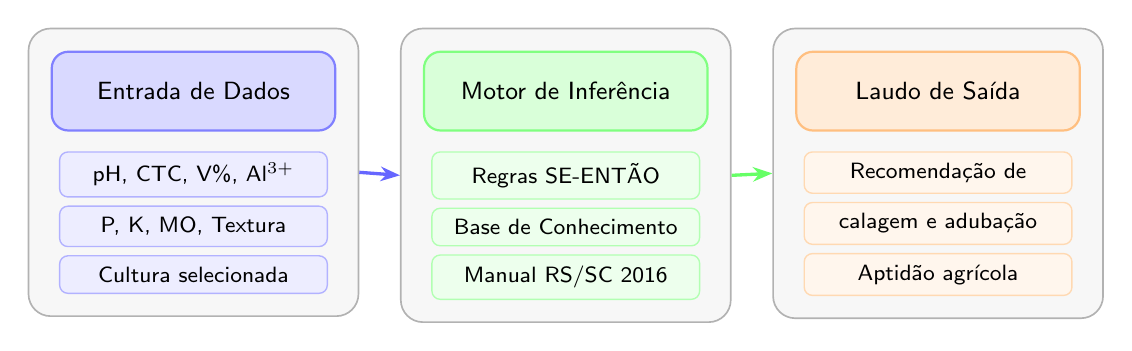
\begin{tikzpicture}[
  node distance = 0.6cm and 1.1cm,
  box/.style = {
    rectangle, rounded corners=6pt,
    minimum width=3.6cm, minimum height=1.0cm,
    text centered, font=\small\sffamily,
    line width=0.8pt
  },
  subbox/.style = {
    rectangle, rounded corners=3pt,
    minimum width=3.4cm,
    text centered, font=\footnotesize\sffamily,
    inner sep=4pt, line width=0.5pt
  },
  arrow/.style = {-{Stealth[length=7pt]}, line width=1.2pt},
  groupbox/.style = {
    rectangle, rounded corners=8pt,
    draw=gray!60, fill=gray!6,
    inner sep=8pt, line width=0.6pt
  }
]
%--- MÓDULO 1: ENTRADA DE DADOS ---
\node[box, fill=blue!15, draw=blue!50] (entrada) {Entrada de Dados};
\node[subbox, fill=blue!7, draw=blue!30, below=0.25cm of entrada] (e1) {pH, CTC, V\%, Al$^{3+}$};
\node[subbox, fill=blue!7, draw=blue!30, below=0.1cm of e1]       (e2) {P, K, MO, Textura};
\node[subbox, fill=blue!7, draw=blue!30, below=0.1cm of e2]       (e3) {Cultura selecionada};
%--- MÓDULO 2: MOTOR DE INFERÊNCIA ---
\node[box, fill=green!15, draw=green!50,
      right=1.1cm of entrada] (motor) {Motor de Inferência};
\node[subbox, fill=green!7, draw=green!30, below=0.25cm of motor] (m1) {Regras SE-ENTÃO};
\node[subbox, fill=green!7, draw=green!30, below=0.1cm of m1]     (m2) {Base de Conhecimento};
\node[subbox, fill=green!7, draw=green!30, below=0.1cm of m2]     (m3) {Manual RS/SC 2016};
%--- MÓDULO 3: LAUDO DE SAÍDA ---
\node[box, fill=orange!15, draw=orange!50,
      right=1.1cm of motor] (saida) {Laudo de Sa\'ida};
\node[subbox, fill=orange!7, draw=orange!30, below=0.25cm of saida] (s1) {Recomenda\c{c}\~ao de};
\node[subbox, fill=orange!7, draw=orange!30, below=0.1cm of s1]     (s2) {calagem e aduba\c{c}\~ao};
\node[subbox, fill=orange!7, draw=orange!30, below=0.1cm of s2]     (s3) {Aptid\~ao agr\'icola};
%--- CAIXAS DE AGRUPAMENTO ---
\begin{scope}[on background layer]
  \node[groupbox, fit=(entrada)(e1)(e2)(e3)] (g1) {};
  \node[groupbox, fit=(motor)(m1)(m2)(m3)]   (g2) {};
  \node[groupbox, fit=(saida)(s1)(s2)(s3)]   (g3) {};
\end{scope}
%--- SETAS ---
\draw[arrow, blue!60]   (g1.east) -- (g2.west);
\draw[arrow, green!60]  (g2.east) -- (g3.west);
\end{tikzpicture}
\caption{\label{fig:arquitetura}Arquitetura conceitual do SIRAS.}
\end{figure}

Do ponto de vista do usuário, a interação com o sistema é direta e
organiza-se em cinco passos, ilustrados na \cref{fig:fluxo}. O usuário
--- técnico agrícola, agrônomo ou produtor --- seleciona a cultura de
interesse, informa em um formulário os resultados de sua análise de
solo, aciona o processamento e, em poucos instantes, recebe na própria
tela o laudo com a recomendação de calagem e adubação e a estimativa de
aptidão, podendo então imprimi-lo ou exportá-lo em PDF. Todo o fluxo
ocorre localmente no navegador, sem necessidade de cadastro ou de
conexão com a internet.

\begin{figure}[htb!]
\centering
\includegraphics[width=\textwidth]{fig/Fluxo_de_Uso_Usuário}
\caption{\label{fig:fluxo}Fluxo de uso do SIRAS na perspectiva do usuário.}
\end{figure}


\subsection{Alternativas Tecnológicas}\label{sec:alternativas}

Caso durante o desenvolvimento sejam identificadas limitações ou necessidades
não previstas nesta proposta, as seguintes alternativas tecnológicas poderão
ser adotadas em substituição ou complemento à stack principal:

\begin{itemize}

  \item \textbf{Django} --- framework web Python mais completo que o Flask,
    indicado caso o sistema evolua para necessitar de autenticação de usuários,
    banco de dados relacional ou administração de dados mais robusta. Mantém
    a linguagem Python, minimizando o reaprendizado;

  \item \textbf{HTML + CSS + JavaScript puro} --- caso seja identificada a
    necessidade de eliminar qualquer dependência de servidor, a lógica de
    recomendação pode ser portada integralmente para JavaScript, resultando
    em uma aplicação que executa diretamente no navegador sem necessidade
    de instalação de Python ou Flask;

  \item \textbf{Streamlit} --- biblioteca Python voltada para criação rápida
    de aplicações de dados com interface web, indicada caso a prioridade
    seja a agilidade no desenvolvimento da interface em detrimento da
    customização visual, pois gera interfaces funcionais com poucas linhas
    de código Python;

  \item \textbf{SQLite} --- banco de dados leve e baseado em arquivo, sem
    necessidade de servidor de banco de dados, indicado caso seja necessário
    persistir histórico de análises realizadas pelo usuário entre sessões
    da aplicação.

\end{itemize}

%-------------------------------------------------------------------
\section{Método}\label{sec:metodo}

O método consiste na sequência de passos descrita a seguir, definida
a partir dos objetivos específicos enunciados na \cref{sec:obj_espec}.

\begin{enumerate}[label=\alph*),leftmargin=3em]

  \item \textbf{Estruturação da base de conhecimento:} extração das
    tabelas de interpretação e recomendação do Manual de Calagem e
    Adubação \citep{ManualCalagem2016} e sua transcrição para arquivos
    JSON, organizados pelos seis grupos de culturas definidos na
    \cref{sec:escopo}, com conferência manual dos valores transcritos;

  \item \textbf{Definição formal das regras:} especificação das regras
    SE-ENTÃO de interpretação dos atributos do solo (classes de
    disponibilidade), do cálculo da necessidade de calagem e do
    dimensionamento das doses de N, P\textsubscript{2}O\textsubscript{5}
    e K\textsubscript{2}O, incluindo os casos especiais das frutíferas
    (três fases), da erva-mate (programas de plantio e de recuperação)
    e do tabaco (tipos Virgínia e Burley);

  \item \textbf{Definição dos critérios de aptidão edáfica:} construção,
    a partir das faixas de interpretação dos atributos químicos e físicos
    do solo estabelecidas no Manual de Calagem e Adubação
    \citep{ManualCalagem2016} e das exigências agronômicas descritas na
    literatura de avaliação de aptidão das terras
    \citep{EmbrapaAptidao2025, Hofig2015}, das faixas de referência
    que sustentarão a classificação de aptidão por cultura, restrita aos
    atributos químicos e físicos do solo;

  \item \textbf{Implementação do módulo de entrada de dados:} formulário
    web para informar os resultados da análise de solo e a cultura de
    interesse, com validação de domínio das variáveis (faixas válidas,
    campos obrigatórios e unidades);

  \item \textbf{Implementação do motor de inferência:} desenvolvimento,
    em Python puro, do mecanismo que aplica as regras da base de
    conhecimento aos dados de entrada;

  \item \textbf{Implementação dos módulos de recomendação e de aptidão:}
    geração das recomendações de calagem e adubação e da estimativa de
    aptidão edáfica, integradas ao laudo de saída renderizado no
    navegador;

  \item \textbf{Construção do conjunto de casos de teste:} elaboração
    dos casos de validação e dos respectivos valores de referência,
    conforme detalhado na \cref{sec:validacao};

  \item \textbf{Validação e análise dos resultados:} execução dos casos
    de teste no sistema, apuração das taxas de concordância, comparação
    com ferramenta existente e decisão sobre as hipóteses formuladas na
    \cref{sec:hipoteses};

  \item \textbf{Avaliação de usabilidade:} aplicação do roteiro de
    tarefas e do questionário SUS com usuários do público-alvo, conforme
    a \cref{sec:val_usabilidade}, e coleta do retorno qualitativo;

  \item \textbf{Redação final:} consolidação da monografia, com a
    discussão dos resultados frente aos trabalhos relacionados, e
    revisão ortográfica e gramatical do texto.

\end{enumerate}

Está prevista a construção de um \textbf{protótipo incremental}, com dois
marcos intermediários de avaliação junto ao orientador: o primeiro
contempla o fluxo completo (entrada, inferência e laudo) restrito ao
grupo de culturas de grãos, cuja lógica de recomendação é uniforme; o
segundo estende o protótipo aos demais grupos, incorporando os casos de
maior complexidade (frutíferas, erva-mate e tabaco). Essa estratégia
permite validar a arquitetura cedo e reduzir o risco de retrabalho.

%-------------------------------------------------------------------
\section{Validação}\label{sec:validacao}

A validação definirá se as hipóteses formuladas na \cref{sec:hipoteses}
serão aceitas ou refutadas. Reconhece-se que a verificação da
concordância com o Manual atesta, sobretudo, que o sistema foi
\emph{implementado corretamente}; por isso, a estratégia de validação é
organizada em três dimensões complementares: (i)~\textbf{correção}, que
verifica a conformidade das saídas com os critérios técnicos de
referência; (ii)~\textbf{comparação}, que posiciona o SIRAS frente a uma
ferramenta existente; e (iii)~\textbf{usabilidade}, que avalia a
experiência de uso com usuários reais.

\subsection{Correção das saídas}\label{sec:val_correcao}

Esta dimensão verifica se as recomendações geradas estão corretas em
relação aos critérios técnicos vigentes. Para evitar métricas
subjetivas, adotam-se as seguintes \textbf{definições operacionais}:

\begin{itemize}

  \item \textbf{Concordância de recomendação:} um caso de teste é
    considerado concordante quando todas as saídas geradas pelo SIRAS
    --- necessidade de calagem (t/ha) e doses de N,
    P\textsubscript{2}O\textsubscript{5} e
    K\textsubscript{2}O (kg/ha) --- coincidem com os valores de
    referência do caso, admitida apenas a tolerância de arredondamento
    decorrente da precisão das tabelas do Manual;

  \item \textbf{Concordância de aptidão:} um caso de teste é considerado
    concordante quando a classe de aptidão edáfica atribuída pelo SIRAS
    coincide com a classe de referência derivada das faixas definidas
    na etapa~c) do método.

\end{itemize}

O conjunto de validação será composto por, no mínimo, \textbf{40 casos
de teste}, estratificados entre os seis grupos de culturas de modo a
cobrir as diferentes classes de interpretação dos atributos (teores
muito baixos a muito altos, diferentes CTCs e texturas) e os casos
especiais de maior complexidade. Os valores de referência de cada caso
constituirão o \textbf{oráculo} da validação e serão obtidos pela
aplicação manual e independente dos critérios do Manual, conferida com
o orientador. Para mitigar o risco de circularidade --- já que o
sistema é construído a partir do mesmo Manual usado na referência ---,
serão priorizados, quando disponíveis, laudos reais de análise de solo
acompanhados de recomendação técnica elaborada por profissional
habilitado, utilizados de forma anonimizada como casos de teste
adicionais.

Como o SIRAS é um sistema determinístico, execuções repetidas de um
mesmo caso produzem sempre a mesma saída; a análise dos resultados,
portanto, não requer testes de comparação de médias, e consistirá na
apuração da \textbf{proporção de casos concordantes} para cada hipótese,
acompanhada do respectivo intervalo de confiança de 95\%. A hipótese
H\textsubscript{1.1} será aceita se a taxa de concordância de
recomendação for igual ou superior a 80\%; a hipótese
H\textsubscript{1.2} será aceita se a taxa de concordância de aptidão
for igual ou superior a 80\%. Os casos discordantes serão analisados
individualmente e discutidos na monografia, distinguindo-se erros de
implementação (corrigíveis) de divergências de interpretação dos
critérios do Manual.

\subsection{Comparação com ferramenta existente}\label{sec:val_comparacao}

Para situar o SIRAS frente ao estado da prática, e seguindo a orientação
de que um artefato de software deve ser comparado a alguma referência
\citep{Wazlawick2014}, um subconjunto dos casos de teste será também
submetido a uma das ferramentas discutidas no \cref{chap:revisao}
--- como o FertFácil \citep{Tiecher2016} ou o AdubaTec
\citep{AdubaTec2021} ---, no que houver sobreposição de funcionalidade,
sobretudo na recomendação de calagem e adubação. Essa comparação é de
natureza \textbf{qualitativa}: pretende evidenciar convergências e
divergências entre as recomendações, documentar as funcionalidades que o
SIRAS oferece e que as ferramentas existentes não contemplam --- em
especial a estimativa de aptidão edáfica integrada à recomendação de
manejo --- e, assim, sustentar a contribuição do trabalho declarada na
H\textsubscript{1.2}. Eventuais divergências serão analisadas à luz das
diferenças de critério ou de versão de Manual adotadas por cada
ferramenta.

\subsection{Usabilidade}\label{sec:val_usabilidade}

A terceira dimensão avalia a experiência de uso do sistema com usuários
reais, aspecto não capturado pelas duas anteriores. Após a conclusão do
protótipo funcional, será conduzida uma avaliação de usabilidade com um
pequeno grupo de participantes do público-alvo (estudantes de agronomia,
técnicos agrícolas ou agrônomos), nos quais cada participante executará
um roteiro de tarefas típicas --- selecionar uma cultura, informar os
dados de uma análise de solo e interpretar o laudo gerado. Ao final, os
participantes responderão ao questionário \textbf{System Usability Scale
(SUS)} \citep{Brooke1996}, instrumento validado e amplamente utilizado
para mensurar a usabilidade percebida, que produz um escore de 0 a 100.
Como referência de interpretação, adota-se o valor consagrado na
literatura da escala, segundo o qual uma pontuação SUS média igual ou
superior a 68 indica usabilidade satisfatória \citep{Brooke1996}.
Complementarmente, será coletado retorno \textbf{qualitativo} por meio
de perguntas abertas sobre dificuldades encontradas e sugestões de
melhoria. Os resultados dessa etapa não testam as hipóteses
H\textsubscript{1.1} e H\textsubscript{1.2}, de natureza técnica, mas
fornecem evidências sobre a adequação da interface ao público-alvo e
subsidiam ajustes finais e recomendações de trabalhos futuros.

%-------------------------------------------------------------------
\section{Cronograma}\label{sec:cronograma}

A \cref{tab:cronograma} apresenta a distribuição das etapas do método
ao longo do período de execução do trabalho, em quinzenas, de agosto ao
início de dezembro de 2026, considerando que a apresentação do trabalho
está prevista para o início de dezembro. As letras correspondem às
etapas detalhadas na \cref{sec:metodo}, e os marcos de protótipo (M1 e
M2) estão indicados nas linhas correspondentes da tabela: M1, ao final
de setembro, corresponde ao fluxo completo restrito ao grupo de grãos;
M2, em meados de outubro, à extensão do protótipo aos demais grupos. A
redação da monografia ocorre de forma contínua a partir da segunda
quinzena de setembro; a validação técnica e a avaliação de usabilidade
concentram-se em novembro, e a primeira quinzena de dezembro fica
reservada à revisão final, entrega e preparação da apresentação.

\begin{table}[htb!]
\centering
\caption{\label{tab:cronograma}Cronograma de execução do trabalho (quinzenas, 2026).}
\small
\begin{tabular}{l c c c c c c c c c}
\hline
 & \multicolumn{2}{c}{\textbf{Ago}} & \multicolumn{2}{c}{\textbf{Set}} & \multicolumn{2}{c}{\textbf{Out}} & \multicolumn{2}{c}{\textbf{Nov}} & \textbf{Dez} \\
\textbf{Etapa} & 1 & 2 & 1 & 2 & 1 & 2 & 1 & 2 & 1 \\
\hline
a) Base de conhecimento (JSON)            & X & X &   &   &   &   &   &   &   \\
b) Regras SE-ENTÃO                        & X & X & X &   &   &   &   &   &   \\
c) Critérios de aptidão edáfica           &   & X & X &   &   &   &   &   &   \\
d) Módulo de entrada de dados             &   & X & X &   &   &   &   &   &   \\
e) Motor de inferência                    &   &   & X & X &   &   &   &   &   \\
\textbf{-- Marco M1 (protótipo grãos)}    &   &   &   & X &   &   &   &   &   \\
f) Módulos de recomendação e aptidão      &   &   &   & X & X &   &   &   &   \\
\textbf{-- Marco M2 (demais grupos)}      &   &   &   &   & X &   &   &   &   \\
g) Casos de teste e oráculo               &   &   &   & X & X & X &   &   &   \\
h) Validação e análise                    &   &   &   &   &   & X & X &   &   \\
i) Avaliação de usabilidade (SUS)         &   &   &   &   &   &   & X & X &   \\
j) Redação da monografia                  &   &   &   & X & X & X & X & X &   \\
k) Revisão final, entrega e apresentação  &   &   &   &   &   &   &   & X & X \\
\hline
\end{tabular}
\end{table}

%-------------------------------------------------------------------
\section{Resultados Esperados}\label{sec:resultados_esperados}

Caso os objetivos sejam alcançados, espera-se dispor de uma ferramenta
funcional, gratuita e executável localmente que apoie técnicos e
produtores do RS na interpretação de análises de solo, na obtenção de
recomendações de calagem e adubação e na avaliação da aptidão edáfica
de culturas específicas, reduzindo erros de interpretação e
qualificando a tomada de decisão. Espera-se, ainda, que a avaliação de
usabilidade indique boa aceitação da interface pelo público-alvo,
confirmando a adequação da ferramenta ao uso pretendido. No contexto do
crédito rural,
espera-se que o SIRAS possa servir de instrumento auxiliar de
conferência das recomendações técnicas que acompanham projetos
agrícolas, conferindo objetividade e rastreabilidade a essa análise.
Em termos de continuidade, a separação entre base de conhecimento e
motor de inferência deverá permitir a extensão futura do sistema a
outras culturas e a manuais de outras regiões, bem como sua utilização
como base para novos trabalhos acadêmicos.

%-------------------------------------------------------------------
\section{Limitações do Estudo}\label{sec:limitacoes}

O trabalho possui as seguintes limitações, que delimitam a abrangência
dos resultados:

\begin{itemize}

  \item a estimativa de aptidão é \textbf{exclusivamente edáfica},
    restrita aos atributos químicos e físicos informados na análise de
    solo, não contemplando fatores de relevo, clima, deficiência
    hídrica ou suscetibilidade à erosão considerados pelos sistemas de
    avaliação regional \citep{EmbrapaAptidao2025, Hofig2015};

  \item o escopo restringe-se às culturas com pH de referência e
    tabelas completas no Manual de Calagem e Adubação para os estados
    do RS e SC \citep{ManualCalagem2016}; culturas como arroz irrigado
    e mandioca, bem como critérios de outras regiões do país, estão
    fora do escopo desta proposta;

  \item a validação será realizada por casos de teste confrontados com
    valores de referência, e não por experimentos agronômicos de campo;
    portanto, os resultados atestam a conformidade do sistema com os
    critérios do Manual, e não o desempenho agronômico das
    recomendações em lavoura;

  \item o SIRAS é uma ferramenta de apoio à decisão e não substitui a
    responsabilidade técnica de profissional habilitado na emissão de
    recomendações oficiais de correção e adubação.

\end{itemize}

Registra-se, ainda, como possibilidade de \textbf{trabalho futuro}, a
implantação do sistema em servidor remoto, de modo a permitir o acesso
diretamente por URL, sem a necessidade de instalação local pelo usuário,
bem como a ampliação do escopo a outras regiões e a avaliação de
usabilidade com amostras maiores de participantes.


%----------------------------------------------------------------
% Referências bibliográficas
%----------------------------------------------------------------
\renewcommand*{\bibname}{\capbib}
\clearpage\phantomsection\addcontentsline{toc}{chapter}{\MakeUppercase{\capbib}}
\bibliography{referencias}

\end{document}
